\documentclass[letterpaper,14pt,titlepage,fleqn]{article}

\setlength{\mathindent}{1cm}

\usepackage{graphicx}                                        

\usepackage{amssymb}                                         
\usepackage{amsmath}                                         
\usepackage{amsthm}                                          

\usepackage{alltt}                                           
\usepackage{float}
\usepackage{color}

\usepackage{url}

\usepackage{balance}
\usepackage[TABBOTCAP, tight]{subfigure}
\usepackage{enumitem}

\usepackage{pstricks, pst-node}

\usepackage{cite}
\usepackage{indentfirst}
\usepackage{listings}

% the following sets the geometry of the page
\usepackage{geometry}
\geometry{textheight=9in, textwidth=6.5in}

% random comment

\newcommand{\cred}[1]{{\color{red}#1}}
\newcommand{\cblue}[1]{{\color{blue}#1}}

\usepackage{hyperref}

\usepackage{textcomp}
\usepackage{listings}

\def\name{Haoxiang Wang; Student ID: 932359049}

%% The following metadata will show up in the PDF properties
\hypersetup{
  colorlinks = true,
  urlcolor = black,
  pdfauthor = {\name},
  pdfkeywords = {CS557 Project 1},
  pdftitle = {Project \#1: Elliptical Dots},
  pdfsubject = {Project \#1: Elliptical Dots},
  pdfpagemode = UseNone
}

\parindent = 0.0 in
\parskip = 0.2 in

\author{\name}
\title{Project \#1: Elliptical Dots}

\begin{document}
\maketitle

This project is the first project I have done in Shaders with RenderMan. I had experience with GLSL in the class CS 550, so this assignment seems pretty easy to handle. It takes me around 2 hours to figure out how RenderMan works and get the project done fitted to all the requirements. The source listing, the results images and the explanation of how code works will be described in the after section. 

\section{Source Listing}
The code for this assignment is almost the same as the example code shown in ``first.rib'' and ``first.sl''. The only different is to implement the ellipses equation in the code. The following code for ``dot.rib'' and ``dot.sl'' shows the way I implement the elliptical dots. The explanation will be done in the next section.\\
\subsection{dot.rib}
\begin{lstlisting}
##RenderMan RIB
version 3.03

# declare the variables:

Declare "Ad" "uniform float"
Declare "Bd" "uniform float"

# define the output file:

Display "dot.tiff" "file" "rgb" 
Format 500 500 -1

# define the lighting:

LightSource "ambientlight" 1 "intensity" [0.25]
LightSource "distantlight" 2 "intensity" [0.75] "from" [5 8 -10] "to" [0 0 0]

# define the rendering parameters:

ShadingRate 1
Projection "perspective" "fov" [70]

# define the scene to be rendered:

WorldBegin
Surface "dot"  "Ad" 0.025  "Bd" 0.10
# specify the surface shader
Color   [1 1 1]				# specify the Cs color
Opacity [1 1 1]				# specify the Os opacity
TransformBegin
Translate 0 0 6			# move away from the eye (= gluLookAt)
Rotate 90  1. 0. 0.		# rotate so don't see north pole
Sphere 3 -3 3 360 		# a full sphere
TransformEnd
WorldEnd

\end{lstlisting}
\subsection{dot.sl}
\begin{lstlisting}
surface
dot(
float	Ad  = 0.025,
Bd = 0.10,
Ks = 0.4,				// specular coefficient
Kd = 0.5, 				// diffuse  coefficient
Ka = 0.1, 				// ambient  coefficient
Roughness = 0.1;			// specular roughness
color	SpecularColor = color( 1, 1, 1 )	// specular color
)
{
color ORANGE = color( 1., .5, 0. );

// be sure the normal points correctly (used for lighting):

varying vector Nf = faceforward( normalize( N ), I );
vector V = normalize( -I );

// determine how many dots over and up we are in right now:

float up = 2. * u;	// because we are rendering a sphere
float vp = v;
float numinu = floor( up / Ad );
float numinv = floor( vp / Bd );
float uc = numinu * Ad + Ad / 2;
float vc = numinv * Bd + Bd / 2;
float test = (up-uc)/(Ad/2)*(up-uc)/(Ad/2) + (vp-vc)/(Bd/2)*(vp-vc)/(Bd/2);

Oi = Os;

//handle the dots:
color TheColor = Cs;
if( test <= 1 )
if( mod( numinu+numinv, 2. ) == 0 )
TheColor = ORANGE;
else
Oi = color( 1., 1., 1. );


// determine the lighted output color Ci:

Ci =        TheColor * Ka * ambient();
Ci = Ci  +  TheColor * Kd * diffuse(Nf);
Ci = Ci  +  SpecularColor * Ks * specular( Nf, V, Roughness );
Ci = Ci * Oi;
}
\end{lstlisting}

\section{Result Images and Explanation}
The two files that I implemented for this assignment is pretty similar to the example files given on the class website. The ``dot.rib'' sets the environment and the pbject, and the ``dot.sl'' files handles the shaders, which puts the elliptical dots on the surface of the sphere.

In the ``dot.rib'' file, I set two uniform variables to pass values to ``dot.sl''. They are ``Ad'' and ``Bd'', which stands for the two diameters for each ellipse. In the ``dot.sl'', these two variables are used to calculate the numbers of ellipses along \textit{u} and \textit{v} directions. The numbers then will be used for calculating each ellipse's center position. Then we can check each pixel to see if it lies in a ellipse by checking the elliptical area around each center point by using ellipse equation: $(\dfrac{u-u_c}{A_r})^2+(\dfrac{v-v_c}{B_r})^2<=1$

If the pixel lies in the elliptical area, the it will be rendered with orange color, otherwise it will be rendered with white. In the example ``first.sl'' file, the opacity is set to 0.6 by setting the $O_i$ to $color(0.6, 0.6, 0.6)$, to disable the transparency, I set the $O_i$ to $color(1., 1., 1.)$ to let the sphere becomes solid white.

The result turns out the two images shown below. The second image shows a different look to the same sphere, by simply change the rotation in the ``dot.rib'' file. Also, the number of the ellipses is larger than the example images in the project description. To change this to less number of dots, we could easily change the values of ``Ad'' and ``Bd'' to some larger number.

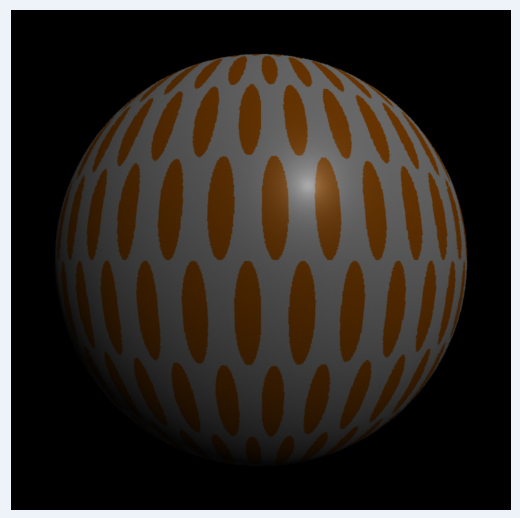
\includegraphics[width=3.2in]{1}
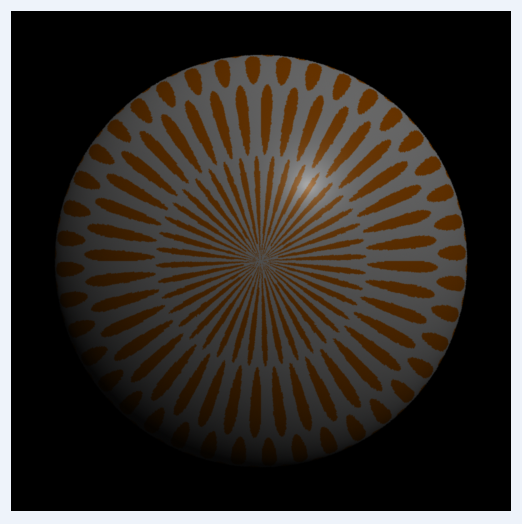
\includegraphics[width=3.2in]{4}

The result turns out great and the code seems easy to handle. However I still had some error images when I was doing the project. The main two mistakes will be using the wrong value in the equation and not using mod operation in the result. The following two images show the error images I have during the programming. The image on the left is the error for using wrong value, and image on the right is the error image for not using mod operation. The reasons for these errors will be explained in the following paragraph.

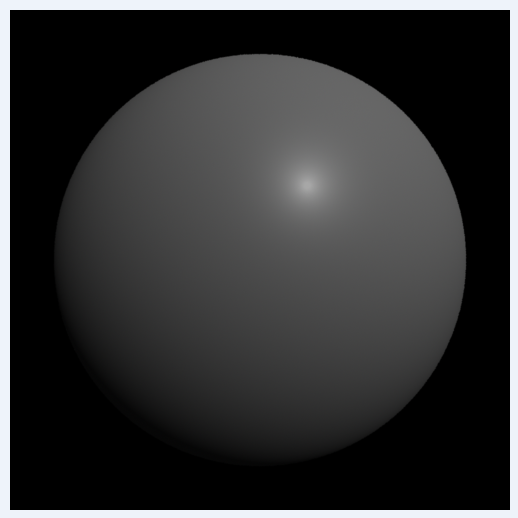
\includegraphics[width=3.2in]{3}
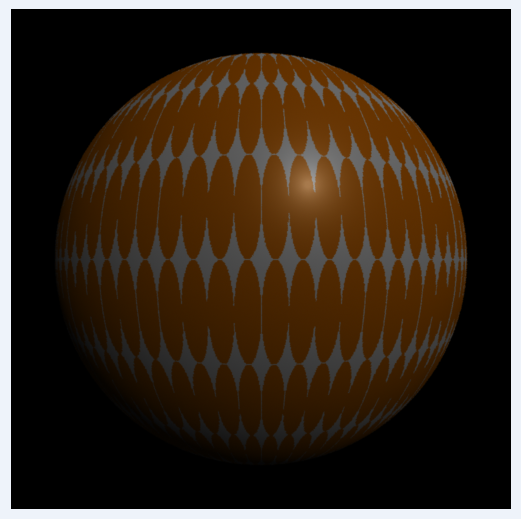
\includegraphics[width=3.2in]{2}

In the ``dot.sl'', the \textit{u} value has been updated to \textit{up} since we are rendering a sphere. However, at the situation I got the error image on the left, I forgot to use \textit{up} instead of \textit{u}. The result turns out the ``test'' values I got are all larger than 1, so that there will be no pixel be considered as in the ellipse, in another words, there will be no orange color rendered on the sphere. This resulted in the whole solid gray sphere as shown in the left image.

The error image on the right shows a sphere covered full of elliptical dots. The reason is that I didn't use mod operation to limit the number of dots rendered on the sphere. The example code we have on the website rendered cheese grid on the sphere surface by check the value of the result of sum up numbers in \textit{u} and \textit{v}. If the result is an even number, then the pixel will be rendered to orange, if the number is an odd number, then the pixel will be left white. I added the same mode operation into the code to limit half number of the dots to white to perform a nicer surface ,and the result turned out pretty good.

\section{Summary}
This first project we have on the Shaders class is a easy one. However even I had some experience in GLSL, I still met some errors during the programming. I learned a lot in this project, and also gained more experience dealing with Shaders. It is also my first time to work with RenderMan, it is pretty interesting and convenient. I'm looking forward to the following projects to create more interesting things.
\end{document}